\section{Bestimmen des Rollreibungskoeffizienten}
Rollt eine Kugel einen bestimmten Weg über den Billardtisch, so entsteht eine der Geschwindigkeit entgegengesetzte
Richtung wirkende Kraft. Die Kraft kann als negative Beschleunigung angegeben werden, wobei diese von einem
Rollreibungskoeffizienten $c_R$ abhängig ist. Das Finden dieses Koeffizienten wird in diesem Kapitel beschrieben.
Die Herleitung und theoretischen Überlegungen finden sich in Kapitel \ref{anhang:herleitung:reibungskoeffizient}.

\begin{figure}[h!]
    \begin{center}
        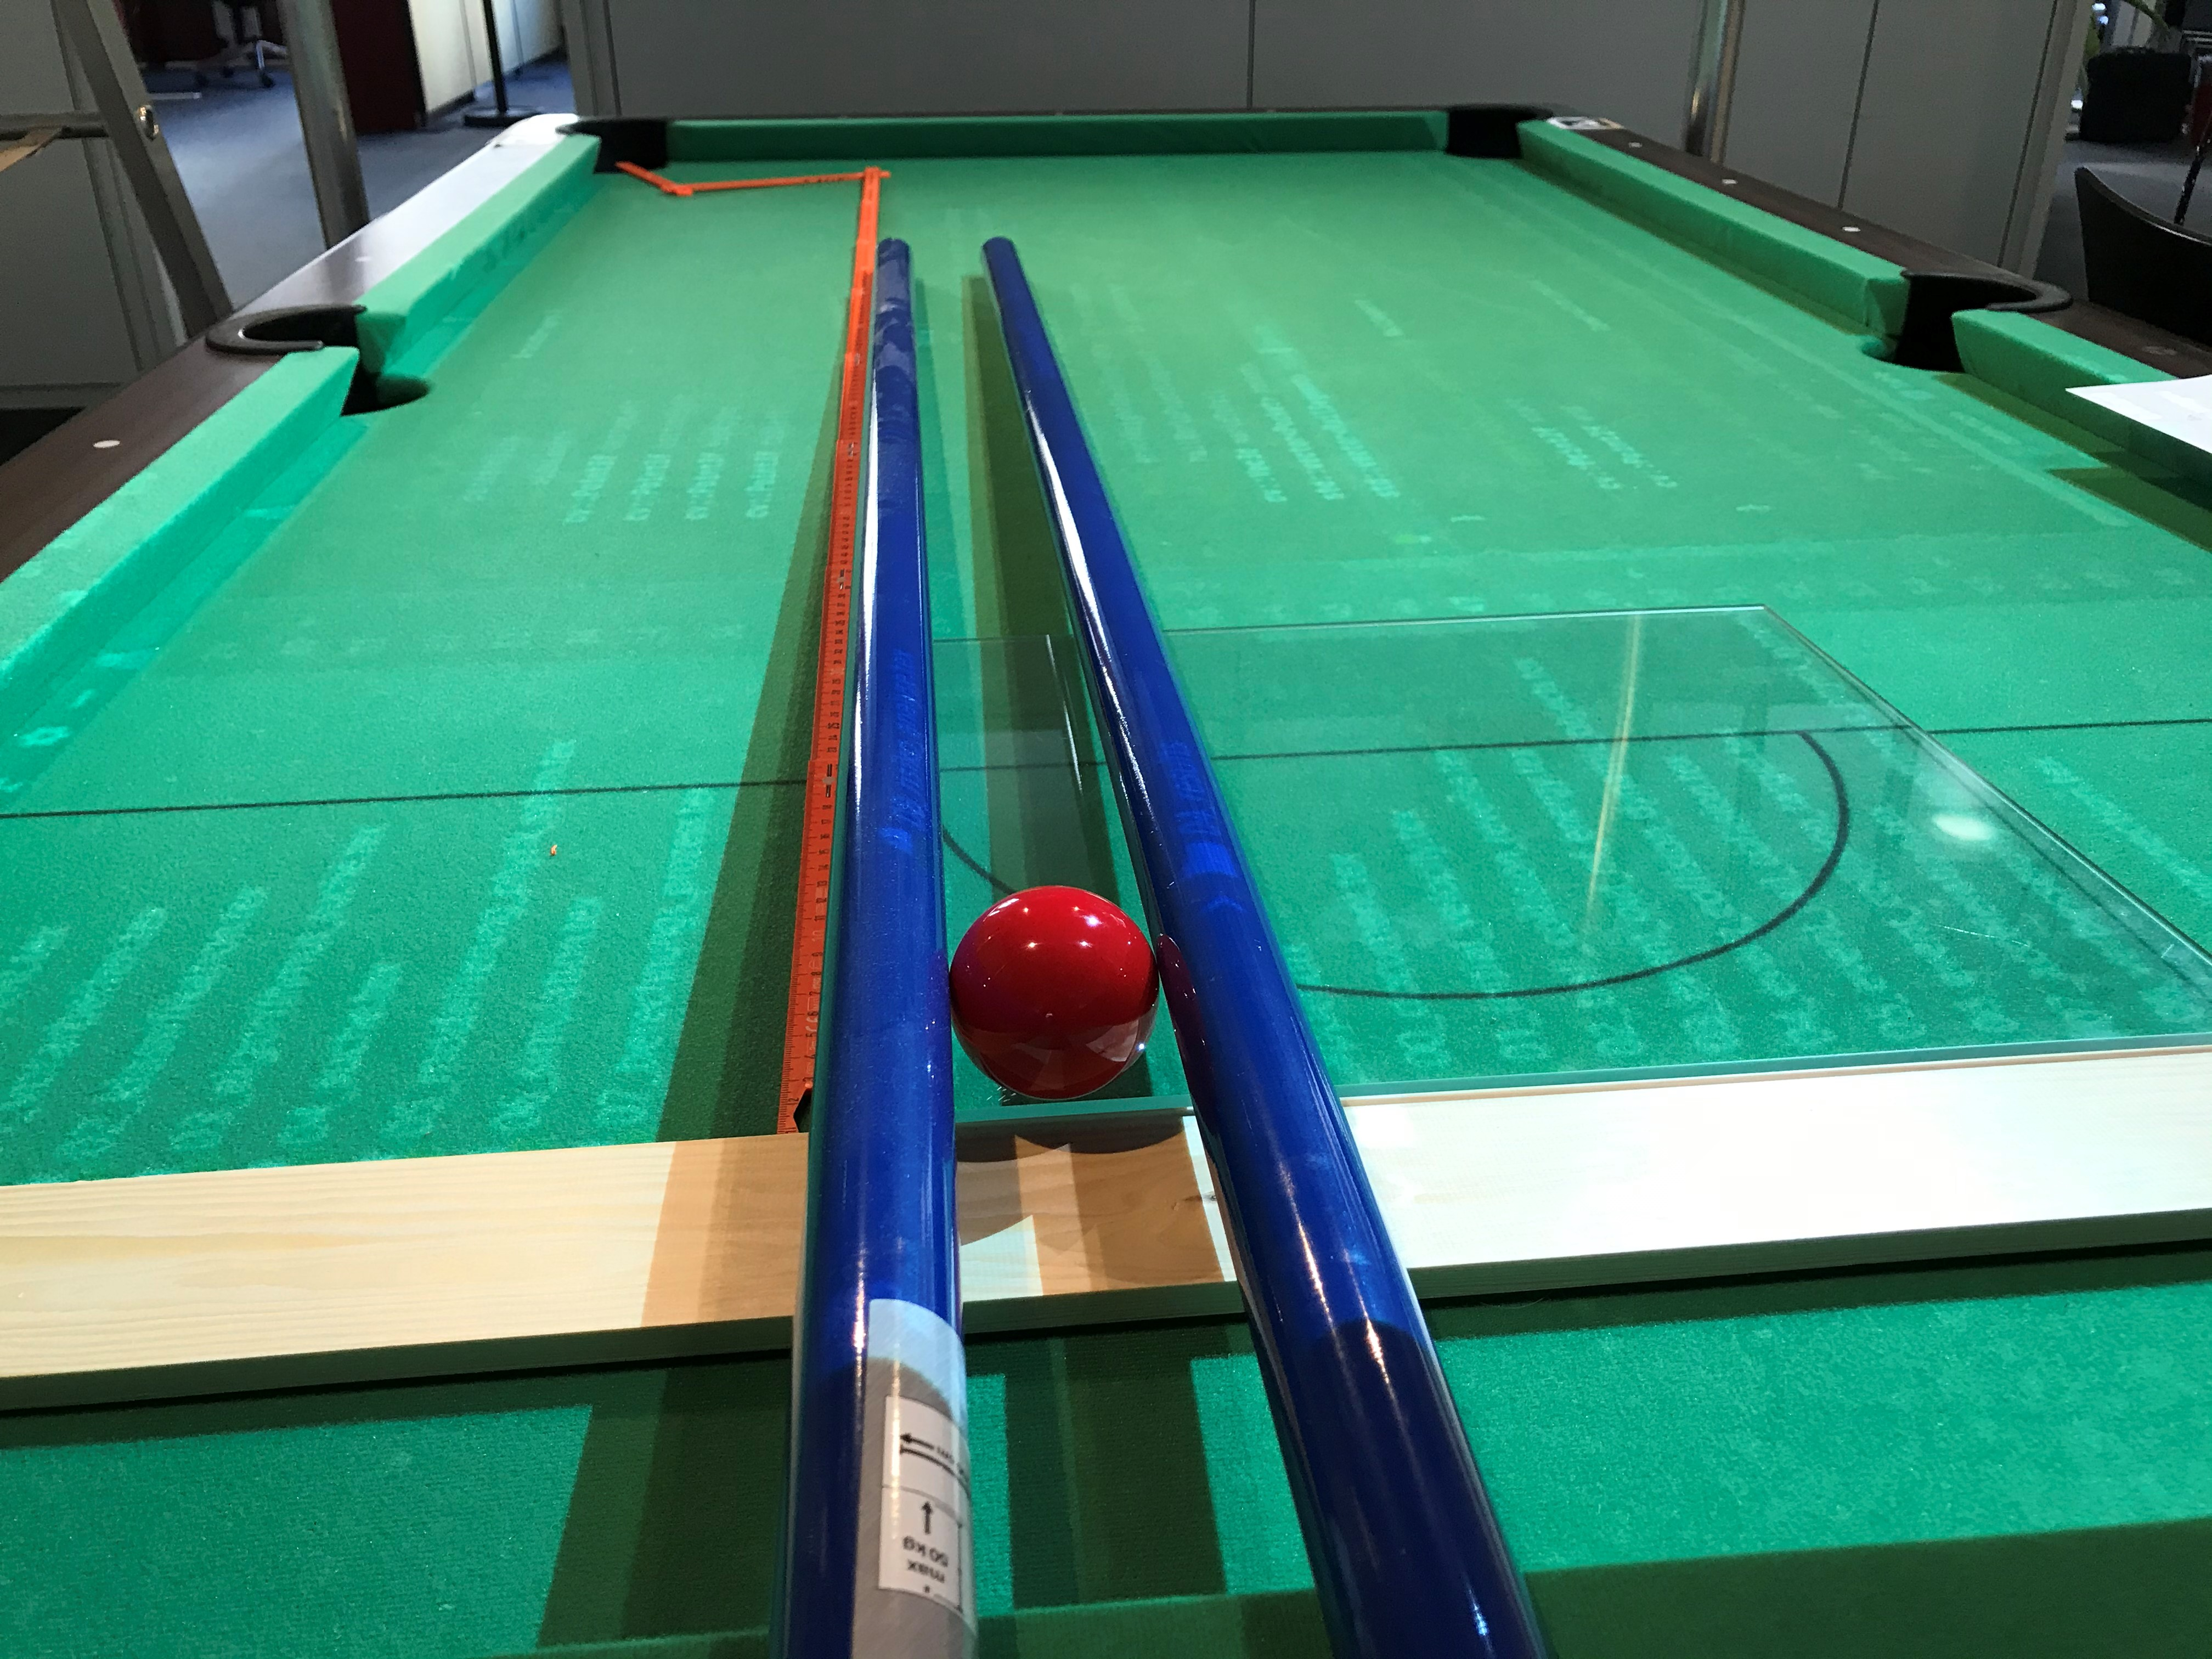
\includegraphics[width=0.5\linewidth]{../common/04_results/resources/00_versuchsaufbau_reibungskoeffizient.png}
    \end{center}
    \caption{Versuchsaufbau zur Bestimmung des Reibungskoeffizienten}
    \label{fig:versuchsaufbau_reibungskoeffizient}
\end{figure}

Abbildung \ref{fig:versuchsaufbau_reibungskoeffizient} veranschaulicht den Versuchsaufbau zur Bestimmung des
Rollreibungskoeffizienten. Wie in Kapitel \ref{anhang:herleitung:reibungskoeffizient} erläutert, muss für die
Rampe ein Material mit möglichst geringer Reibung verwendet werden, weswegen die Wahl auf Glas fiel.
Weiterhin wird der Weg der Kugel geführt, da sie eine möglichst gerade Bahn rollen muss. Die so entstehende Reibung
an der Bahn wird ebenfalls vernachlässigt.

Es wurden zwei Versuche durchgeführt mit unterschiedlicher Höhe der Rampe. Die Ergebnisse dieser Messungen wie
deren Median sind in der Tabelle \ref{tab:distanzmessungen_rollende_kugel} aufgeführt.

\begin{table}[ht]
    \rowcolors{1}{\seccolor!10}{\seccolor!10} % Rows with 10% of secondary color
    \begin{tabular}{ccc}
        \rowcolor{\seccolor!50}
        \textbf{Distanz {[}mm{]} \textbackslash Höhe {[}mm{]}} & \textbf{13}  & \textbf{19}   \\\bfhmidline
        & 957          & 1228          \\\bfhmidline
        & 949          & 1253          \\\bfhmidline
        & 926          & 1263          \\\bfhmidline
        & 914          & 1280          \\\bfhmidline
        & 931          & 1281          \\\bfhmidline
        & 932          & 1296          \\\bfhmidline
        & 941          & 1256          \\\bfhmidline
        & 926          & 1295          \\\bfhmidline
        & 931          & 1295          \\\bfhmidline
        & 941          & 1304          \\\bfhmidline
        & 943          & 1314          \\\bfhmidline
        & 937          & 1316          \\\bfhmidline
        & 947          & 1284          \\\bfhmidline
        & 949          & 1303          \\\bfhmidline
        & 947          & 1319          \\\bfhmidline
        & -            & 1320          \\\bfhmidline
        \textbf{Median} & \textbf{941} & \textbf{1295} \\\bfhmidline
    \end{tabular}
    \caption{Ergebnisse Distanzmessung einer rollenden Kugel}
    \label{tab:distanzmessungen_rollende_kugel}
\end{table}

Anhand des Ablaufs aus Kapitel \ref{anhang:herleitung:reibungskoeffizient} können die Reibungskoeffizienten aus
Tabelle \ref{tab:reibungskoeffizienten} bestimmt werden. Daraus wird der Mittelwert berechnet, welcher das Resultat
bildet.

\begin{table}[ht]
    \rowcolors{1}{\seccolor!10}{\seccolor!10} % Rows with 10% of secondary color
    \begin{tabular}{cc}
        \rowcolor{\seccolor!50}
        \textbf{Strecke {[}mm{]}} & \textbf{Reibungskoeffizient} \\\bfhmidline
        941                       & 0.0138151                    \\\bfhmidline
        1295                      & 0.0146718                    \\\bfhmidline
        \textbf{Mittelwert}       & 0.0142435                    \\\bfhmidline
    \end{tabular}
    \caption{Reibungskoeffizienten über Strecke}
    \label{tab:reibungskoeffizienten}
\end{table}